\section{Zielsetzung}
In diesem Versuch soll der Photoeffekt untersucht werden, wie zum Beispiel die Elektronenenergie von der Wellenlänge des Lichts abhängt.

\section{Theorie}
\label{sec:Theorie}
Um den Photoeffekt erklären zu können, wird das Korpuskelmodell, ein Grenzfall der Quantenelektrodynamik betrachtet.
In diesem Modell wird davon ausgegangen, dass die Energie des Lichts durch Photonen im Raum bewegt wird.
Nach Einstein sind diese Korpuskeln gleichzusetzen mit den Planckschen Energiequanten.

Der Photoeffekt wird untersucht indem eine Festkörperoberfläche im Vakuum mit monochromatischem Licht bestrahlt wird, diese Elektrode wird als Photkathode bezeichnet.
Gegenüber der Photkathode befindet sich eine weitere Elektrode mit entgegengesetztem Potential.
Diese Anordnung, siehe \autoref{fig:anordnung}} ist an ein Strommessgerät verbunden

\begin{figure}
    \centering
    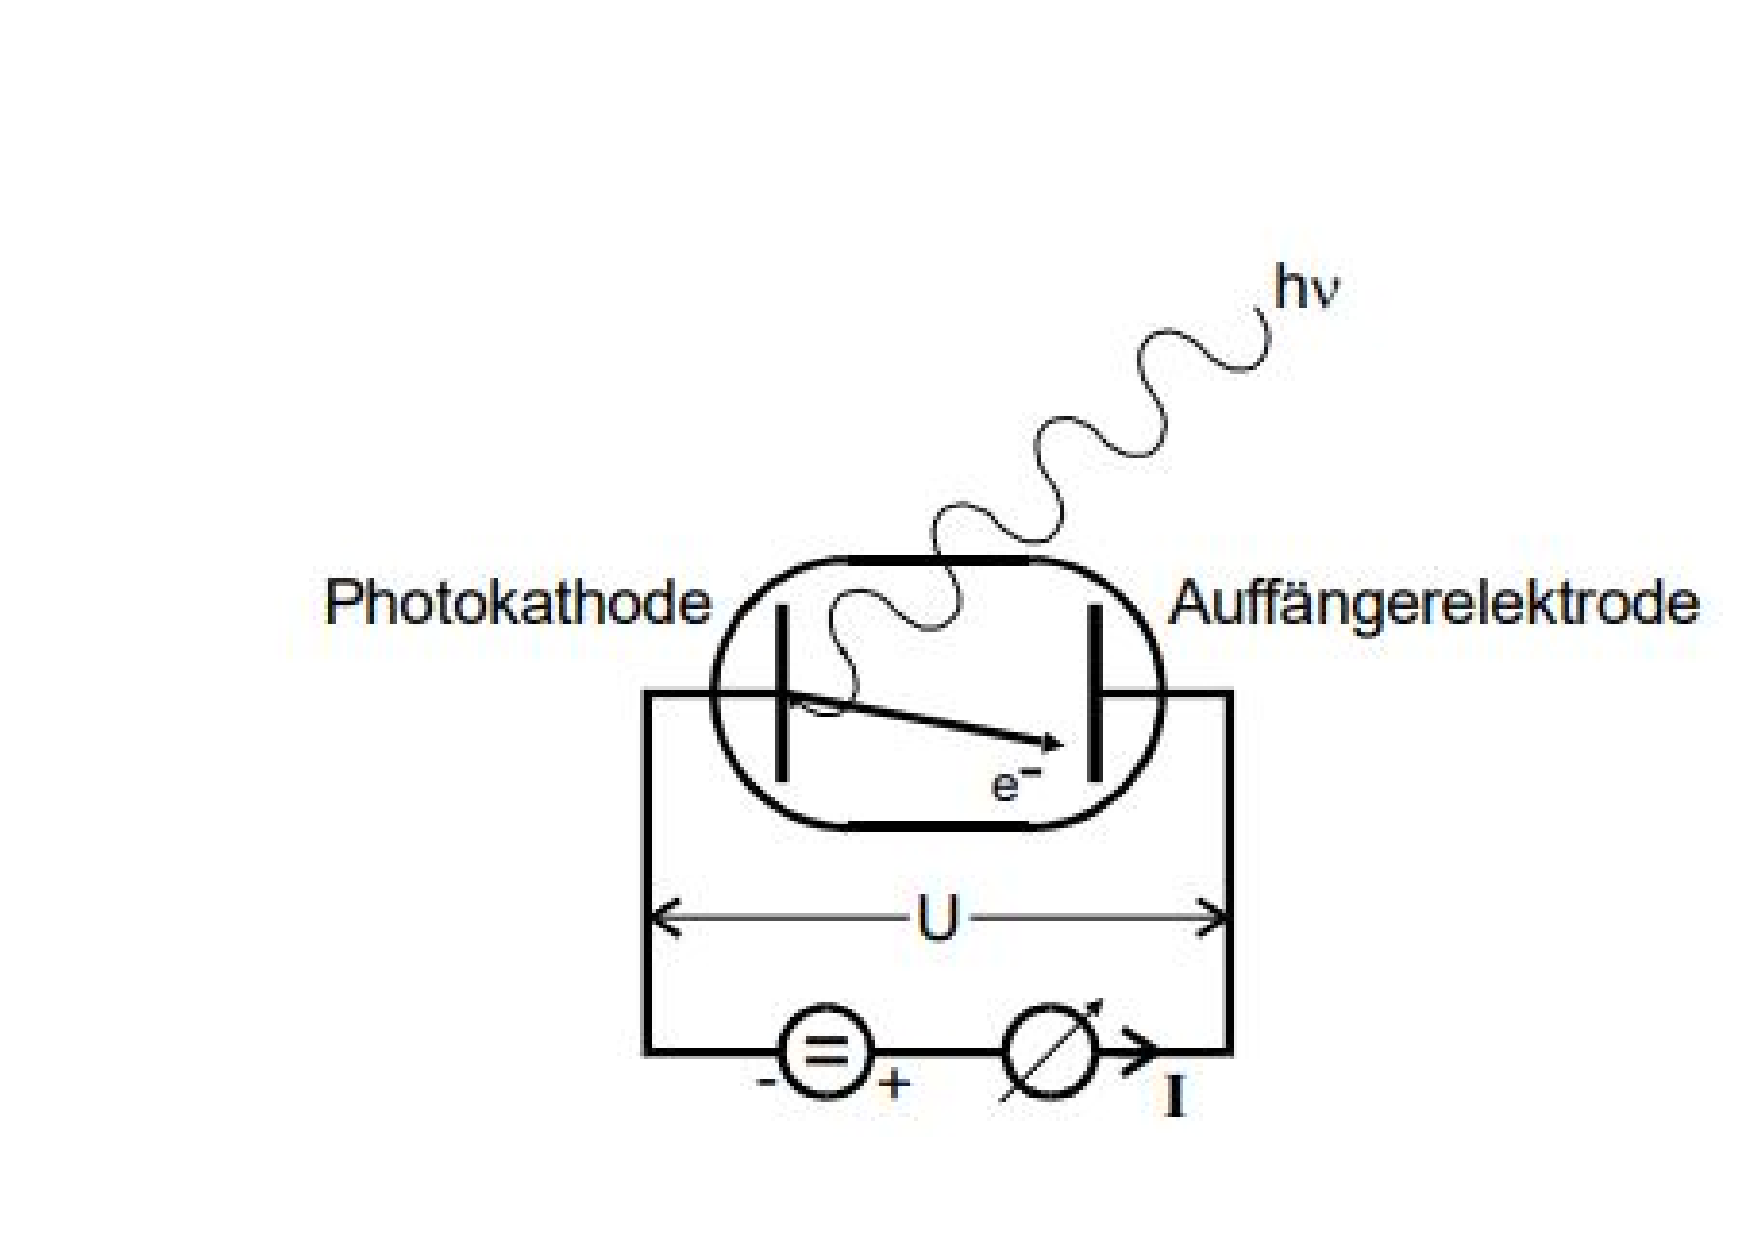
\includegraphics[width =\textwidth]{content/anordnung.pdf}
    \caption{Anordnung zur Untersuchung des Photoeffekts.\cite{anleitung}}
    \label{fig:anordnung}
\end{figure}

Die zu beobachten Ergebnisse aus diesem Experiment sind zum einen, dass die Zahl der ausgelösten Elektronen pro Zeiteinheit proportional zur Lichtintesität ist.
Dies ist damit zu begründen, dass die Zahl der Photonen pro Zeit- und Raumwinkeleinheit proportional zur Lichtintensität ist.
Zusätzlich kann ein Photon auch nur ein Elektron auslösen.

Ein weiteres Ergebnis ist, dass die kinetische Energie der Photonen proportional zur Lichtfrequenz $\nu$ ist und insbesondere unabhängig von der Lichtintensität.
Die Photonenenergie wird vollständig auf des Elektron übertragen, genaugenommen in die Austrittsarbeit $A_\text{k}$ zum Verlassen der Oberfläche und in die kinetische Energie $E_\text{kin}$.
Die Energie des Photons hängt dabei nur von der Frequenz $\nu$ und dem Planckschen Wirkungsquantum $\symup{h}$ ab.
Die Energiebilanz lautet demnach:
\begin{equation}
    \label{eqn:Energiebilanz}
    \symup{h} \nu = E_\text{kin} + A_\text{k}.
\end{equation}
An \autoref{eqn:Energiebilanz} ist auch das dritte Ergebnis erkennbar, der Photoeffekt tritt ab einer bestimmten Grenzfrequenz auf.
Folgendes Verhältnis muss also gelten:
\begin{equation*}
    \symup{h} \nu > A_\text{k},
\end{equation*}
denn sonst ist die Energie nicht groß genug um die Austrittsarbeit zu verrichten.
Es werden also keine Elektronen aus der Oberfläche gelöst.

\subsection{Experimentelle Untersuchung des Photoeffekts}
\label{subsec:Experimentelle Untersuchung des Photoeffekts mit der Gegenfeldmethode}

Zur Untersuchung wird ein evakuierter Glaskolben, der zwei Elektroden enthählt, verwendet.
Diese sogenannte Photozelle ist in \autoref{fig:photozelle} zu sehen.
Im Inneren der Photozelle befindet sich eine Photokathode aus einer aufgedampften Metall- oder Legierungsschicht, diese wird vom Licht bestrahlt.
Um sie herum ist ein ringförmiger Anodendraht, der parallel zur Photokathodenoberfläche liegt.

\begin{figure}
    \centering
    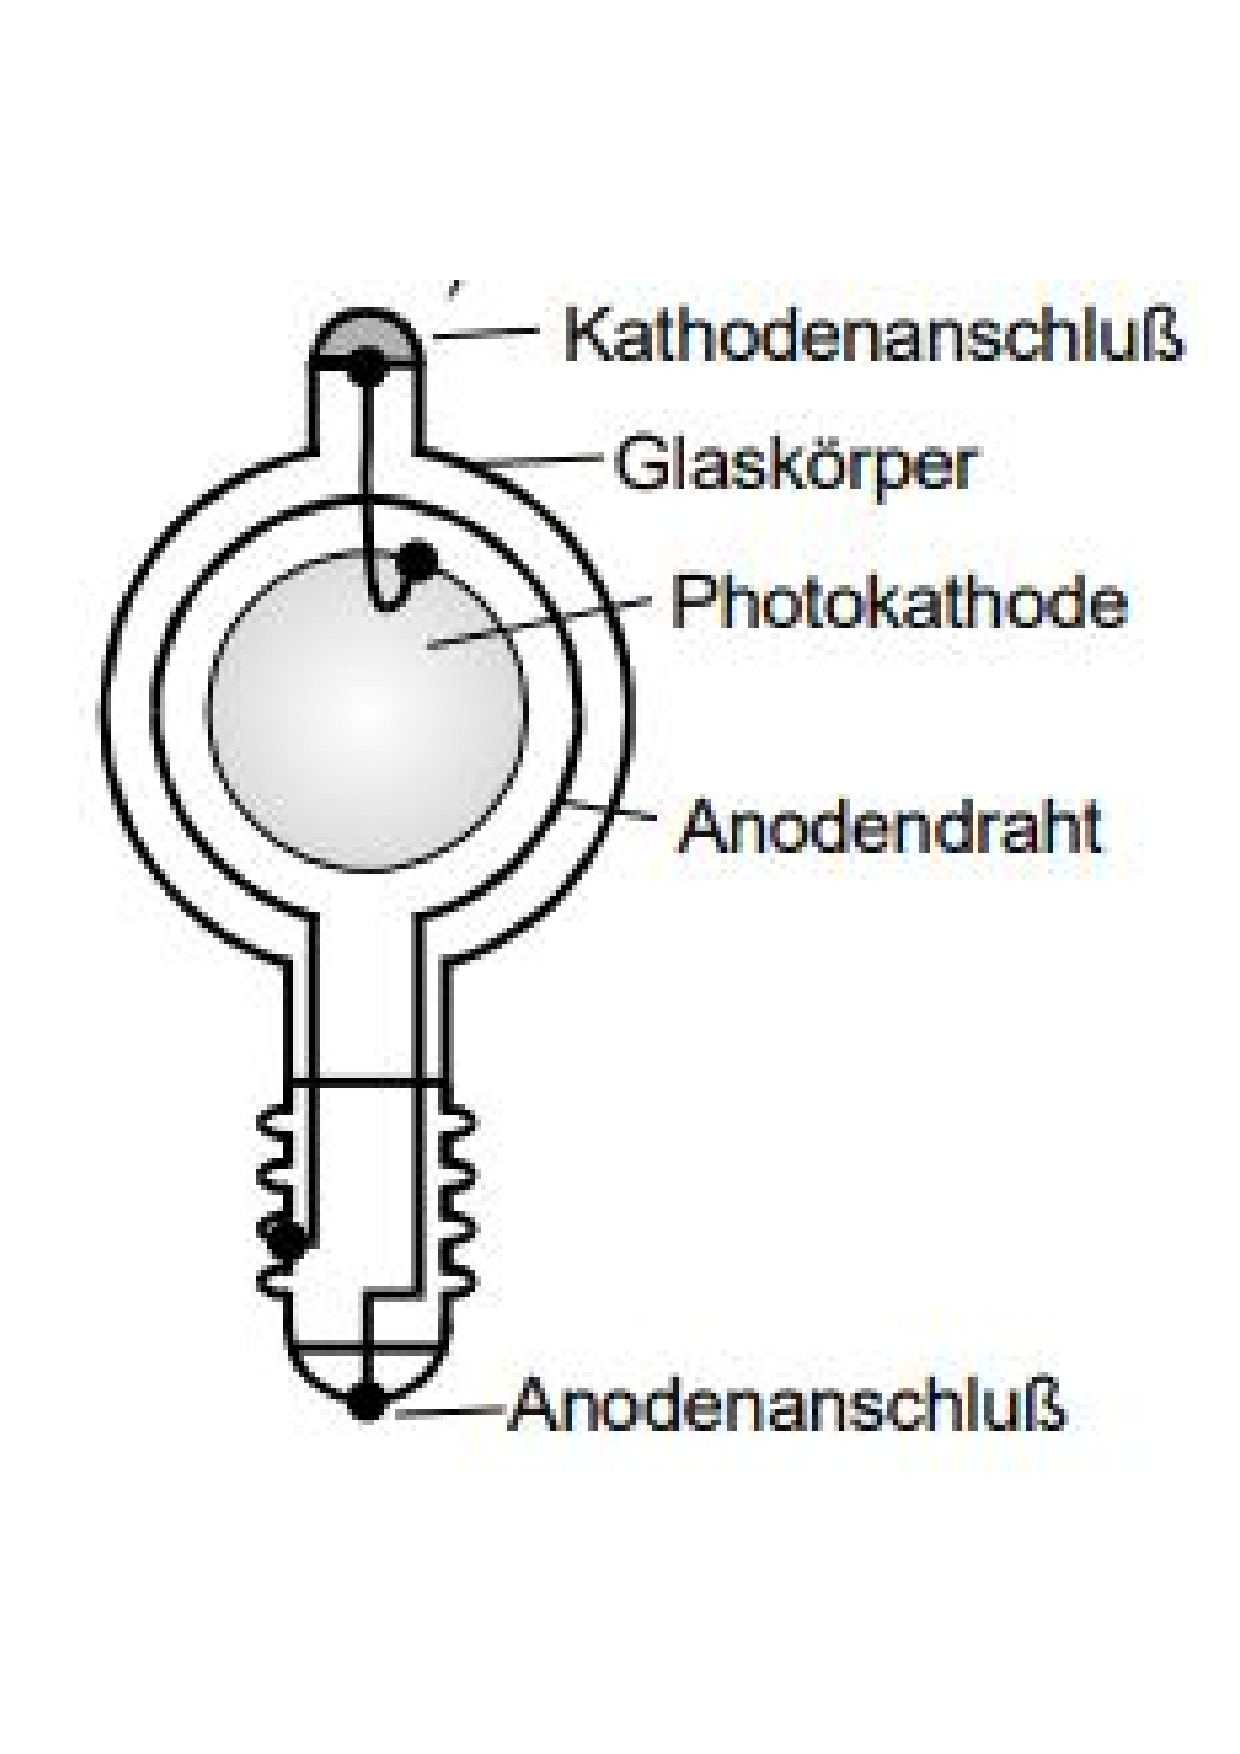
\includegraphics[width =\textwidth]{content/photozelle.pdf}
    \caption{Aufbau einer Photozelle.\cite{anleitung}}
    \label{fig:photozelle}
\end{figure}

\begin{figure}
    \centering
    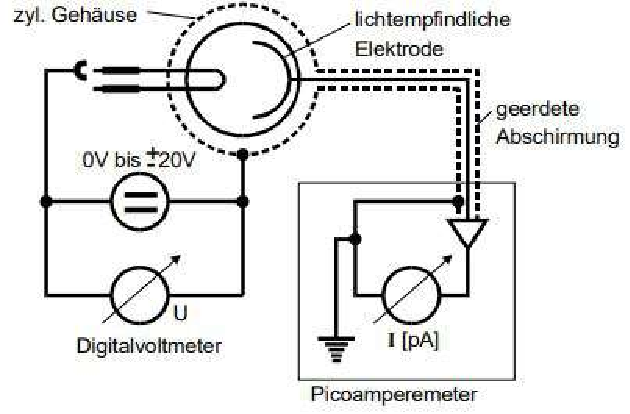
\includegraphics[width =\textwidth]{content/schaltbild.pdf}
    \caption{Schaltbild der Messaparatur.\cite{anleitung}}
    \label{fig:schaltbild}
\end{figure}

Die Photozelle aus \autoref{fig:photozelle} ist an ein digitales Voltmeter und an ein Picoamperemeter angeschlossen, siehe \autoref{fig:schaltbild}.
Eine variable Spannung $U$ wird zwischen die Elektroden angelegt, dadurch entsteht ein Potential, das die gelösten Elektronen abbremst.
Mit dem Picoamperemeter wird der Strom, der von der Photokathode zur Anode fließt, gemessen.
Die gelösten Elektronen, die die Anode erreichen, haben eine kinetische Energie größer als $\text{e}_0 U$.
Der Strom verschwindet dann, wenn 

\begin{equation}
    \symup{e}_0 U_g = \frac{1}{2} \text{m}_0 v^2_\text{max}.
    \label{eqn:stromgrenze}
\end{equation}

Hierbei ist $\symup{e}_0$ die Elementarladung, $\symup{m}_0$ die Ruhemasse des Elektrons und $v_\text{max}$ die Geschwindigkeit der schnellsten Elektronen.
Die kinetische Energie der schnellsten Elektronen kann aus der Gegenspannung $U_g$ bestimmt werden.
Es gilt nach \autoref{eqn:Energiebilanz} und \autoref{eqn:stromgrenze} :

\begin{equation}
    \symup{h} \nu = \symup{e}_0 U_g + A_k
\end{equation}

Bei der Untersuchung einer Strom-Spannungskurve wie in ... wird ersichtlich, dass der Photostrom bei $U = U_g$ nicht sofort abbricht.
Der Strom sinkt vorher erkennbar.
Der Grund ist, dass die ausgelösten Elektronen schon im Festkörper, also vor der Auslösung unterschiedliche Energien haben.
Somit sind diese Photoelektronen nicht genau monoenergetisch, sondern haben eine Energieverteilung von 0 bis zu $\frac{1}{2} m_0 v^2_max$.
Die Fermi-Dirac-Statistik macht über diese Energieverteilung der Elektronen im Festkörper eine Aussage.
Die Elektronenenergie kann zwischen 0 und $\xi$  betragen, dabei ist die Fermi-Energie $\xi$ einige $eV$ groß.
Unter bestimmten Voraussetzungen besteht zwischen dem Photostrom $I_\text{Ph}$ und der Bremsspannung $U$ ein parabolischer Zusammenhang:
\begin{equation*}
    I_{Ph} \propto U^2.
\end{equation*}
Eine weitere Grund von einem nicht vorhandenen Photostrom ist, dass die Austrittsarbeit $A_A$ am Anodenmetall größer als die Photonenenergie $\symup{h} \nu$ ist.
Die gelösten Elektronen müssen dann gegen das Gegenfeld laufen, um die Anode zu erreichen.
Wird eine Beschleunigungsspannnung $U_b$ angelegt, ist ein Photostrom messbar.
Es gilt:
\begin{equation}
    \symup{h} \nu + \symup{e}_0 U_b \geq A_A.
\end{equation}